\documentclass[ignorenonframetext,]{beamer}
\setbeamertemplate{caption}[numbered]
\setbeamertemplate{caption label separator}{: }
\setbeamercolor{caption name}{fg=normal text.fg}
\beamertemplatenavigationsymbolsempty
\usepackage{lmodern}
\usepackage{amssymb,amsmath}
\usepackage{ifxetex,ifluatex}
\usepackage{fixltx2e} % provides \textsubscript
\ifnum 0\ifxetex 1\fi\ifluatex 1\fi=0 % if pdftex
  \usepackage[T1]{fontenc}
  \usepackage[utf8]{inputenc}
\else % if luatex or xelatex
  \ifxetex
    \usepackage{mathspec}
  \else
    \usepackage{fontspec}
  \fi
  \defaultfontfeatures{Ligatures=TeX,Scale=MatchLowercase}
\fi
% use upquote if available, for straight quotes in verbatim environments
\IfFileExists{upquote.sty}{\usepackage{upquote}}{}
% use microtype if available
\IfFileExists{microtype.sty}{%
\usepackage{microtype}
\UseMicrotypeSet[protrusion]{basicmath} % disable protrusion for tt fonts
}{}
\newif\ifbibliography
\hypersetup{
            pdftitle={Module 9: The Multivariate Normal Distribution},
            pdfauthor={Rebecca C. Steorts},
            pdfborder={0 0 0},
            breaklinks=true}
\urlstyle{same}  % don't use monospace font for urls
\usepackage{color}
\usepackage{fancyvrb}
\newcommand{\VerbBar}{|}
\newcommand{\VERB}{\Verb[commandchars=\\\{\}]}
\DefineVerbatimEnvironment{Highlighting}{Verbatim}{commandchars=\\\{\}}
% Add ',fontsize=\small' for more characters per line
\usepackage{framed}
\definecolor{shadecolor}{RGB}{248,248,248}
\newenvironment{Shaded}{\begin{snugshade}}{\end{snugshade}}
\newcommand{\KeywordTok}[1]{\textcolor[rgb]{0.13,0.29,0.53}{\textbf{#1}}}
\newcommand{\DataTypeTok}[1]{\textcolor[rgb]{0.13,0.29,0.53}{#1}}
\newcommand{\DecValTok}[1]{\textcolor[rgb]{0.00,0.00,0.81}{#1}}
\newcommand{\BaseNTok}[1]{\textcolor[rgb]{0.00,0.00,0.81}{#1}}
\newcommand{\FloatTok}[1]{\textcolor[rgb]{0.00,0.00,0.81}{#1}}
\newcommand{\ConstantTok}[1]{\textcolor[rgb]{0.00,0.00,0.00}{#1}}
\newcommand{\CharTok}[1]{\textcolor[rgb]{0.31,0.60,0.02}{#1}}
\newcommand{\SpecialCharTok}[1]{\textcolor[rgb]{0.00,0.00,0.00}{#1}}
\newcommand{\StringTok}[1]{\textcolor[rgb]{0.31,0.60,0.02}{#1}}
\newcommand{\VerbatimStringTok}[1]{\textcolor[rgb]{0.31,0.60,0.02}{#1}}
\newcommand{\SpecialStringTok}[1]{\textcolor[rgb]{0.31,0.60,0.02}{#1}}
\newcommand{\ImportTok}[1]{#1}
\newcommand{\CommentTok}[1]{\textcolor[rgb]{0.56,0.35,0.01}{\textit{#1}}}
\newcommand{\DocumentationTok}[1]{\textcolor[rgb]{0.56,0.35,0.01}{\textbf{\textit{#1}}}}
\newcommand{\AnnotationTok}[1]{\textcolor[rgb]{0.56,0.35,0.01}{\textbf{\textit{#1}}}}
\newcommand{\CommentVarTok}[1]{\textcolor[rgb]{0.56,0.35,0.01}{\textbf{\textit{#1}}}}
\newcommand{\OtherTok}[1]{\textcolor[rgb]{0.56,0.35,0.01}{#1}}
\newcommand{\FunctionTok}[1]{\textcolor[rgb]{0.00,0.00,0.00}{#1}}
\newcommand{\VariableTok}[1]{\textcolor[rgb]{0.00,0.00,0.00}{#1}}
\newcommand{\ControlFlowTok}[1]{\textcolor[rgb]{0.13,0.29,0.53}{\textbf{#1}}}
\newcommand{\OperatorTok}[1]{\textcolor[rgb]{0.81,0.36,0.00}{\textbf{#1}}}
\newcommand{\BuiltInTok}[1]{#1}
\newcommand{\ExtensionTok}[1]{#1}
\newcommand{\PreprocessorTok}[1]{\textcolor[rgb]{0.56,0.35,0.01}{\textit{#1}}}
\newcommand{\AttributeTok}[1]{\textcolor[rgb]{0.77,0.63,0.00}{#1}}
\newcommand{\RegionMarkerTok}[1]{#1}
\newcommand{\InformationTok}[1]{\textcolor[rgb]{0.56,0.35,0.01}{\textbf{\textit{#1}}}}
\newcommand{\WarningTok}[1]{\textcolor[rgb]{0.56,0.35,0.01}{\textbf{\textit{#1}}}}
\newcommand{\AlertTok}[1]{\textcolor[rgb]{0.94,0.16,0.16}{#1}}
\newcommand{\ErrorTok}[1]{\textcolor[rgb]{0.64,0.00,0.00}{\textbf{#1}}}
\newcommand{\NormalTok}[1]{#1}
\usepackage{graphicx,grffile}
\makeatletter
\def\maxwidth{\ifdim\Gin@nat@width>\linewidth\linewidth\else\Gin@nat@width\fi}
\def\maxheight{\ifdim\Gin@nat@height>\textheight0.8\textheight\else\Gin@nat@height\fi}
\makeatother
% Scale images if necessary, so that they will not overflow the page
% margins by default, and it is still possible to overwrite the defaults
% using explicit options in \includegraphics[width, height, ...]{}
\setkeys{Gin}{width=\maxwidth,height=\maxheight,keepaspectratio}

% Prevent slide breaks in the middle of a paragraph:
\widowpenalties 1 10000
\raggedbottom

\AtBeginPart{
  \let\insertpartnumber\relax
  \let\partname\relax
  \frame{\partpage}
}
\AtBeginSection{
  \ifbibliography
  \else
    \let\insertsectionnumber\relax
    \let\sectionname\relax
    \frame{\sectionpage}
  \fi
}
\AtBeginSubsection{
  \let\insertsubsectionnumber\relax
  \let\subsectionname\relax
  \frame{\subsectionpage}
}

\setlength{\parindent}{0pt}
\setlength{\parskip}{6pt plus 2pt minus 1pt}
\setlength{\emergencystretch}{3em}  % prevent overfull lines
\providecommand{\tightlist}{%
  \setlength{\itemsep}{0pt}\setlength{\parskip}{0pt}}
\setcounter{secnumdepth}{0}
% Custom definitions
% To use this customization file, insert the line "% Custom definitions
% To use this customization file, insert the line "% Custom definitions
% To use this customization file, insert the line "% Custom definitions
% To use this customization file, insert the line "\input{custom}" in the header of the tex file.

% Formatting

\tolerance=1000
\usepackage[margin=1in]{geometry}


% Packages

% \usepackage{amssymb,latexsym}
\usepackage{amssymb,amsfonts,amsmath,latexsym,amsthm}
%\usepackage[usenames,dvipsnames]{color}
\usepackage[]{graphicx}
\usepackage[space]{grffile}
\usepackage{mathrsfs}   % fancy math font
% \usepackage[font=small,skip=0pt]{caption}
\usepackage[skip=0pt]{caption}
\usepackage{subcaption}
\usepackage{verbatim}
\usepackage{url}
\usepackage{bm}
\usepackage{dsfont}
\usepackage{extarrows}
\usepackage{multirow}
% \usepackage{wrapfig}
% \usepackage{epstopdf}
\usepackage{rotating}
\usepackage{tikz}
\usetikzlibrary{fit}					% fitting shapes to coordinates
%\usetikzlibrary{backgrounds}	% drawing the background after the foreground


% \usepackage[dvipdfm,colorlinks,citecolor=blue,linkcolor=blue,urlcolor=blue]{hyperref}
\usepackage[colorlinks,citecolor=blue,linkcolor=blue,urlcolor=blue]{hyperref}
%\usepackage{hyperref}
\usepackage[authoryear,round]{natbib}


%  Theorems, etc.

\theoremstyle{plain}
\newtheorem{theorem}{Theorem}[section]
\newtheorem{corollary}[theorem]{Corollary}
\newtheorem{lemma}[theorem]{Lemma}
\newtheorem{proposition}[theorem]{Proposition}
\newtheorem{condition}[theorem]{Condition}
% \newtheorem{conditions}[theorem]{Conditions}

\theoremstyle{definition}
\newtheorem{definition}[theorem]{Definition}
% \newtheorem*{unnumbered-definition}{Definition}
\newtheorem{example}[theorem]{Example}
\theoremstyle{remark}
\newtheorem*{remark}{Remark}
\numberwithin{equation}{section}




% Document-specific shortcuts
\newcommand{\btheta}{{\bm\theta}}
\newcommand{\bbtheta}{{\pmb{\bm\theta}}}

\newcommand{\commentary}[1]{\ifx\showcommentary\undefined\else \emph{#1}\fi}

\newcommand{\term}[1]{\textit{\textbf{#1}}}

% Math shortcuts

% Probability distributions
\DeclareMathOperator*{\Exp}{Exp}
\DeclareMathOperator*{\TExp}{TExp}
\DeclareMathOperator*{\Bernoulli}{Bernoulli}
\DeclareMathOperator*{\Beta}{Beta}
\DeclareMathOperator*{\Ga}{Gamma}
\DeclareMathOperator*{\TGamma}{TGamma}
\DeclareMathOperator*{\Poisson}{Poisson}
\DeclareMathOperator*{\Binomial}{Binomial}
\DeclareMathOperator*{\NormalGamma}{NormalGamma}
\DeclareMathOperator*{\InvGamma}{InvGamma}
\DeclareMathOperator*{\Cauchy}{Cauchy}
\DeclareMathOperator*{\Uniform}{Uniform}
\DeclareMathOperator*{\Gumbel}{Gumbel}
\DeclareMathOperator*{\Pareto}{Pareto}
\DeclareMathOperator*{\Mono}{Mono}
\DeclareMathOperator*{\Geometric}{Geometric}
\DeclareMathOperator*{\Wishart}{Wishart}

% Math operators
\DeclareMathOperator*{\argmin}{arg\,min}
\DeclareMathOperator*{\argmax}{arg\,max}
\DeclareMathOperator*{\Cov}{Cov}
\DeclareMathOperator*{\diag}{diag}
\DeclareMathOperator*{\median}{median}
\DeclareMathOperator*{\Vol}{Vol}

% Math characters
\newcommand{\R}{\mathbb{R}}
\newcommand{\Z}{\mathbb{Z}}
\newcommand{\E}{\mathbb{E}}
\renewcommand{\Pr}{\mathbb{P}}
\newcommand{\I}{\mathds{1}}
\newcommand{\V}{\mathbb{V}}

\newcommand{\A}{\mathcal{A}}
\newcommand{\C}{\mathcal{C}}
\newcommand{\D}{\mathcal{D}}
\newcommand{\Hcal}{\mathcal{H}}
\newcommand{\M}{\mathcal{M}}
\newcommand{\N}{\mathcal{N}}
\newcommand{\X}{\mathcal{X}}
\newcommand{\Zcal}{\mathcal{Z}}
\renewcommand{\P}{\mathcal{P}}

\newcommand{\T}{\mathtt{T}}
\renewcommand{\emptyset}{\varnothing}


% Miscellaneous commands
\newcommand{\iid}{\stackrel{\mathrm{iid}}{\sim}}
\newcommand{\matrixsmall}[1]{\bigl(\begin{smallmatrix}#1\end{smallmatrix} \bigr)}

\newcommand{\items}[1]{\begin{itemize} #1 \end{itemize}}

\newcommand{\todo}[1]{\emph{\textcolor{red}{(#1)}}}

\newcommand{\branch}[4]{
\left\{
	\begin{array}{ll}
		#1  & \mbox{if } #2 \\
		#3 & \mbox{if } #4
	\end{array}
\right.
}

% approximately proportional to
\def\app#1#2{%
  \mathrel{%
    \setbox0=\hbox{$#1\sim$}%
    \setbox2=\hbox{%
      \rlap{\hbox{$#1\propto$}}%
      \lower1.3\ht0\box0%
    }%
    \raise0.25\ht2\box2%
  }%
}
\def\approxprop{\mathpalette\app\relax}

% \newcommand{\approptoinn}[2]{\mathrel{\vcenter{
  % \offinterlineskip\halign{\hfil$##$\cr
    % #1\propto\cr\noalign{\kern2pt}#1\sim\cr\noalign{\kern-2pt}}}}}

% \newcommand{\approxpropto}{\mathpalette\approptoinn\relax}





" in the header of the tex file.

% Formatting

\tolerance=1000
\usepackage[margin=1in]{geometry}


% Packages

% \usepackage{amssymb,latexsym}
\usepackage{amssymb,amsfonts,amsmath,latexsym,amsthm}
%\usepackage[usenames,dvipsnames]{color}
\usepackage[]{graphicx}
\usepackage[space]{grffile}
\usepackage{mathrsfs}   % fancy math font
% \usepackage[font=small,skip=0pt]{caption}
\usepackage[skip=0pt]{caption}
\usepackage{subcaption}
\usepackage{verbatim}
\usepackage{url}
\usepackage{bm}
\usepackage{dsfont}
\usepackage{extarrows}
\usepackage{multirow}
% \usepackage{wrapfig}
% \usepackage{epstopdf}
\usepackage{rotating}
\usepackage{tikz}
\usetikzlibrary{fit}					% fitting shapes to coordinates
%\usetikzlibrary{backgrounds}	% drawing the background after the foreground


% \usepackage[dvipdfm,colorlinks,citecolor=blue,linkcolor=blue,urlcolor=blue]{hyperref}
\usepackage[colorlinks,citecolor=blue,linkcolor=blue,urlcolor=blue]{hyperref}
%\usepackage{hyperref}
\usepackage[authoryear,round]{natbib}


%  Theorems, etc.

\theoremstyle{plain}
\newtheorem{theorem}{Theorem}[section]
\newtheorem{corollary}[theorem]{Corollary}
\newtheorem{lemma}[theorem]{Lemma}
\newtheorem{proposition}[theorem]{Proposition}
\newtheorem{condition}[theorem]{Condition}
% \newtheorem{conditions}[theorem]{Conditions}

\theoremstyle{definition}
\newtheorem{definition}[theorem]{Definition}
% \newtheorem*{unnumbered-definition}{Definition}
\newtheorem{example}[theorem]{Example}
\theoremstyle{remark}
\newtheorem*{remark}{Remark}
\numberwithin{equation}{section}




% Document-specific shortcuts
\newcommand{\btheta}{{\bm\theta}}
\newcommand{\bbtheta}{{\pmb{\bm\theta}}}

\newcommand{\commentary}[1]{\ifx\showcommentary\undefined\else \emph{#1}\fi}

\newcommand{\term}[1]{\textit{\textbf{#1}}}

% Math shortcuts

% Probability distributions
\DeclareMathOperator*{\Exp}{Exp}
\DeclareMathOperator*{\TExp}{TExp}
\DeclareMathOperator*{\Bernoulli}{Bernoulli}
\DeclareMathOperator*{\Beta}{Beta}
\DeclareMathOperator*{\Ga}{Gamma}
\DeclareMathOperator*{\TGamma}{TGamma}
\DeclareMathOperator*{\Poisson}{Poisson}
\DeclareMathOperator*{\Binomial}{Binomial}
\DeclareMathOperator*{\NormalGamma}{NormalGamma}
\DeclareMathOperator*{\InvGamma}{InvGamma}
\DeclareMathOperator*{\Cauchy}{Cauchy}
\DeclareMathOperator*{\Uniform}{Uniform}
\DeclareMathOperator*{\Gumbel}{Gumbel}
\DeclareMathOperator*{\Pareto}{Pareto}
\DeclareMathOperator*{\Mono}{Mono}
\DeclareMathOperator*{\Geometric}{Geometric}
\DeclareMathOperator*{\Wishart}{Wishart}

% Math operators
\DeclareMathOperator*{\argmin}{arg\,min}
\DeclareMathOperator*{\argmax}{arg\,max}
\DeclareMathOperator*{\Cov}{Cov}
\DeclareMathOperator*{\diag}{diag}
\DeclareMathOperator*{\median}{median}
\DeclareMathOperator*{\Vol}{Vol}

% Math characters
\newcommand{\R}{\mathbb{R}}
\newcommand{\Z}{\mathbb{Z}}
\newcommand{\E}{\mathbb{E}}
\renewcommand{\Pr}{\mathbb{P}}
\newcommand{\I}{\mathds{1}}
\newcommand{\V}{\mathbb{V}}

\newcommand{\A}{\mathcal{A}}
\newcommand{\C}{\mathcal{C}}
\newcommand{\D}{\mathcal{D}}
\newcommand{\Hcal}{\mathcal{H}}
\newcommand{\M}{\mathcal{M}}
\newcommand{\N}{\mathcal{N}}
\newcommand{\X}{\mathcal{X}}
\newcommand{\Zcal}{\mathcal{Z}}
\renewcommand{\P}{\mathcal{P}}

\newcommand{\T}{\mathtt{T}}
\renewcommand{\emptyset}{\varnothing}


% Miscellaneous commands
\newcommand{\iid}{\stackrel{\mathrm{iid}}{\sim}}
\newcommand{\matrixsmall}[1]{\bigl(\begin{smallmatrix}#1\end{smallmatrix} \bigr)}

\newcommand{\items}[1]{\begin{itemize} #1 \end{itemize}}

\newcommand{\todo}[1]{\emph{\textcolor{red}{(#1)}}}

\newcommand{\branch}[4]{
\left\{
	\begin{array}{ll}
		#1  & \mbox{if } #2 \\
		#3 & \mbox{if } #4
	\end{array}
\right.
}

% approximately proportional to
\def\app#1#2{%
  \mathrel{%
    \setbox0=\hbox{$#1\sim$}%
    \setbox2=\hbox{%
      \rlap{\hbox{$#1\propto$}}%
      \lower1.3\ht0\box0%
    }%
    \raise0.25\ht2\box2%
  }%
}
\def\approxprop{\mathpalette\app\relax}

% \newcommand{\approptoinn}[2]{\mathrel{\vcenter{
  % \offinterlineskip\halign{\hfil$##$\cr
    % #1\propto\cr\noalign{\kern2pt}#1\sim\cr\noalign{\kern-2pt}}}}}

% \newcommand{\approxpropto}{\mathpalette\approptoinn\relax}





" in the header of the tex file.

% Formatting

\tolerance=1000
\usepackage[margin=1in]{geometry}


% Packages

% \usepackage{amssymb,latexsym}
\usepackage{amssymb,amsfonts,amsmath,latexsym,amsthm}
%\usepackage[usenames,dvipsnames]{color}
\usepackage[]{graphicx}
\usepackage[space]{grffile}
\usepackage{mathrsfs}   % fancy math font
% \usepackage[font=small,skip=0pt]{caption}
\usepackage[skip=0pt]{caption}
\usepackage{subcaption}
\usepackage{verbatim}
\usepackage{url}
\usepackage{bm}
\usepackage{dsfont}
\usepackage{extarrows}
\usepackage{multirow}
% \usepackage{wrapfig}
% \usepackage{epstopdf}
\usepackage{rotating}
\usepackage{tikz}
\usetikzlibrary{fit}					% fitting shapes to coordinates
%\usetikzlibrary{backgrounds}	% drawing the background after the foreground


% \usepackage[dvipdfm,colorlinks,citecolor=blue,linkcolor=blue,urlcolor=blue]{hyperref}
\usepackage[colorlinks,citecolor=blue,linkcolor=blue,urlcolor=blue]{hyperref}
%\usepackage{hyperref}
\usepackage[authoryear,round]{natbib}


%  Theorems, etc.

\theoremstyle{plain}
\newtheorem{theorem}{Theorem}[section]
\newtheorem{corollary}[theorem]{Corollary}
\newtheorem{lemma}[theorem]{Lemma}
\newtheorem{proposition}[theorem]{Proposition}
\newtheorem{condition}[theorem]{Condition}
% \newtheorem{conditions}[theorem]{Conditions}

\theoremstyle{definition}
\newtheorem{definition}[theorem]{Definition}
% \newtheorem*{unnumbered-definition}{Definition}
\newtheorem{example}[theorem]{Example}
\theoremstyle{remark}
\newtheorem*{remark}{Remark}
\numberwithin{equation}{section}




% Document-specific shortcuts
\newcommand{\btheta}{{\bm\theta}}
\newcommand{\bbtheta}{{\pmb{\bm\theta}}}

\newcommand{\commentary}[1]{\ifx\showcommentary\undefined\else \emph{#1}\fi}

\newcommand{\term}[1]{\textit{\textbf{#1}}}

% Math shortcuts

% Probability distributions
\DeclareMathOperator*{\Exp}{Exp}
\DeclareMathOperator*{\TExp}{TExp}
\DeclareMathOperator*{\Bernoulli}{Bernoulli}
\DeclareMathOperator*{\Beta}{Beta}
\DeclareMathOperator*{\Ga}{Gamma}
\DeclareMathOperator*{\TGamma}{TGamma}
\DeclareMathOperator*{\Poisson}{Poisson}
\DeclareMathOperator*{\Binomial}{Binomial}
\DeclareMathOperator*{\NormalGamma}{NormalGamma}
\DeclareMathOperator*{\InvGamma}{InvGamma}
\DeclareMathOperator*{\Cauchy}{Cauchy}
\DeclareMathOperator*{\Uniform}{Uniform}
\DeclareMathOperator*{\Gumbel}{Gumbel}
\DeclareMathOperator*{\Pareto}{Pareto}
\DeclareMathOperator*{\Mono}{Mono}
\DeclareMathOperator*{\Geometric}{Geometric}
\DeclareMathOperator*{\Wishart}{Wishart}

% Math operators
\DeclareMathOperator*{\argmin}{arg\,min}
\DeclareMathOperator*{\argmax}{arg\,max}
\DeclareMathOperator*{\Cov}{Cov}
\DeclareMathOperator*{\diag}{diag}
\DeclareMathOperator*{\median}{median}
\DeclareMathOperator*{\Vol}{Vol}

% Math characters
\newcommand{\R}{\mathbb{R}}
\newcommand{\Z}{\mathbb{Z}}
\newcommand{\E}{\mathbb{E}}
\renewcommand{\Pr}{\mathbb{P}}
\newcommand{\I}{\mathds{1}}
\newcommand{\V}{\mathbb{V}}

\newcommand{\A}{\mathcal{A}}
\newcommand{\C}{\mathcal{C}}
\newcommand{\D}{\mathcal{D}}
\newcommand{\Hcal}{\mathcal{H}}
\newcommand{\M}{\mathcal{M}}
\newcommand{\N}{\mathcal{N}}
\newcommand{\X}{\mathcal{X}}
\newcommand{\Zcal}{\mathcal{Z}}
\renewcommand{\P}{\mathcal{P}}

\newcommand{\T}{\mathtt{T}}
\renewcommand{\emptyset}{\varnothing}


% Miscellaneous commands
\newcommand{\iid}{\stackrel{\mathrm{iid}}{\sim}}
\newcommand{\matrixsmall}[1]{\bigl(\begin{smallmatrix}#1\end{smallmatrix} \bigr)}

\newcommand{\items}[1]{\begin{itemize} #1 \end{itemize}}

\newcommand{\todo}[1]{\emph{\textcolor{red}{(#1)}}}

\newcommand{\branch}[4]{
\left\{
	\begin{array}{ll}
		#1  & \mbox{if } #2 \\
		#3 & \mbox{if } #4
	\end{array}
\right.
}

% approximately proportional to
\def\app#1#2{%
  \mathrel{%
    \setbox0=\hbox{$#1\sim$}%
    \setbox2=\hbox{%
      \rlap{\hbox{$#1\propto$}}%
      \lower1.3\ht0\box0%
    }%
    \raise0.25\ht2\box2%
  }%
}
\def\approxprop{\mathpalette\app\relax}

% \newcommand{\approptoinn}[2]{\mathrel{\vcenter{
  % \offinterlineskip\halign{\hfil$##$\cr
    % #1\propto\cr\noalign{\kern2pt}#1\sim\cr\noalign{\kern-2pt}}}}}

% \newcommand{\approxpropto}{\mathpalette\approptoinn\relax}





" in the header of the tex file.

% Formatting

\setbeamertemplate{navigation symbols}{}
\setbeamertemplate{footline}[page number]


% Packages
\usepackage{amssymb,amsfonts,amsmath,latexsym,amsthm}
%\usepackage[usenames,dvipsnames]{color}
%\usepackage[]{graphicx}
%\usepackage[space]{grffile}
\usepackage{mathrsfs} 
 \usepackage{amssymb,latexsym}
\usepackage{amssymb,amsfonts,amsmath,latexsym,amsthm, bm}
%\usepackage[usenames,dvipsnames]{color}
%\usepackage[]{graphicx}
%\usepackage[space]{grffile}
\usepackage{mathrsfs}   % fancy math font
% \usepackage[font=small,skip=0pt]{caption}
%\usepackage[skip=0pt]{caption}
%\usepackage{subcaption}
%\usepackage{verbatim}
%\usepackage{url}
%\usepackage{bm}
\usepackage{dsfont}
\usepackage{multirow}
%\usepackage{extarrows}
%\usepackage{multirow}
%% \usepackage{wrapfig}
%% \usepackage{epstopdf}
%\usepackage{rotating}
%\usepackage{tikz}
%\usetikzlibrary{fit}					% fitting shapes to coordinates
%\usetikzlibrary{backgrounds}	% drawing the background after the foreground


% \usepackage[dvipdfm,colorlinks,citecolor=blue,linkcolor=blue,urlcolor=blue]{hyperref}
%\usepackage[colorlinks,citecolor=blue,linkcolor=blue,urlcolor=blue]{hyperref}
%%\usepackage{hyperref}
%\usepackage[authoryear,round]{natbib}


%  Theorems, etc.

%\theoremstyle{plain}
%\newtheorem{theorem}{Theorem}[section]
%\newtheorem{corollary}[theorem]{Corollary}
%\newtheorem{lemma}[theorem]{Lemma}
%\newtheorem{proposition}[theorem]{Proposition}
%\newtheorem{condition}[theorem]{Condition}
% \newtheorem{conditions}[theorem]{Conditions}

%\theoremstyle{definition}
%\newtheorem{definition}[theorem]{Definition}
%% \newtheorem*{unnumbered-definition}{Definition}
%\newtheorem{example}[theorem]{Example}
%\theoremstyle{remark}
%\newtheorem*{remark}{Remark}
%\numberwithin{equation}{section}






% Document-specific shortcuts
\newcommand{\btheta}{{\bm\theta}}
\newcommand{\bbtheta}{{\pmb{\bm\theta}}}

\newcommand{\commentary}[1]{\ifx\showcommentary\undefined\else \emph{#1}\fi}

\newcommand{\term}[1]{\textit{\textbf{#1}}}

% Math shortcuts

% Probability distributions
\DeclareMathOperator*{\Exp}{Exp}
\DeclareMathOperator*{\TExp}{TExp}
\DeclareMathOperator*{\Bernoulli}{Bernoulli}
\DeclareMathOperator*{\Beta}{Beta}
\DeclareMathOperator*{\Ga}{Gamma}
\DeclareMathOperator*{\TGamma}{TGamma}
\DeclareMathOperator*{\Poisson}{Poisson}
\DeclareMathOperator*{\Binomial}{Binomial}
\DeclareMathOperator*{\NormalGamma}{NormalGamma}
\DeclareMathOperator*{\InvGamma}{InvGamma}
\DeclareMathOperator*{\Cauchy}{Cauchy}
\DeclareMathOperator*{\Uniform}{Uniform}
\DeclareMathOperator*{\Gumbel}{Gumbel}
\DeclareMathOperator*{\Pareto}{Pareto}
\DeclareMathOperator*{\Mono}{Mono}
\DeclareMathOperator*{\Geometric}{Geometric}
\DeclareMathOperator*{\Wishart}{Wishart}

% Math operators
\DeclareMathOperator*{\argmin}{arg\,min}
\DeclareMathOperator*{\argmax}{arg\,max}
\DeclareMathOperator*{\Cov}{Cov}
\DeclareMathOperator*{\diag}{diag}
\DeclareMathOperator*{\median}{median}
\DeclareMathOperator*{\Vol}{Vol}

% Math characters
\newcommand{\R}{\mathbb{R}}
\newcommand{\Z}{\mathbb{Z}}
\newcommand{\E}{\mathbb{E}}
\renewcommand{\Pr}{\mathbb{P}}
\newcommand{\I}{\mathds{1}}
\newcommand{\V}{\mathbb{V}}

\newcommand{\A}{\mathcal{A}}
%\newcommand{\C}{\mathcal{C}}
\newcommand{\D}{\mathcal{D}}
\newcommand{\Hcal}{\mathcal{H}}
\newcommand{\M}{\mathcal{M}}
\newcommand{\N}{\mathcal{N}}
\newcommand{\X}{\mathcal{X}}
\newcommand{\Zcal}{\mathcal{Z}}
\renewcommand{\P}{\mathcal{P}}

\newcommand{\T}{\mathtt{T}}
\renewcommand{\emptyset}{\varnothing}

\newcommand{\bmu}{\bm{\mu}}
\newcommand{\bX}   {\bm{X}}
\newcommand{\bY}   {\bm{Y}}
\newcommand{\sig}   {\Sigma}
\newcommand{\bx}{\ensuremath{\mathbf{X}}}
%\newcommand{\X}{\ensuremath{\mathbf{x}}}
%\newcommand{\w}{\ensuremath{\mathbf{w}}}
%\newcommand{\h}{\ensuremath{\mathbf{h}}}
%\newcommand{\V}{\ensuremath{\mathbf{v}}}
%\newcommand{\cov}{\text{Cov}}
\newcommand{\var}{\text{Var}}


% Miscellaneous commands
\newcommand{\iid}{\stackrel{\mathrm{iid}}{\sim}}
\newcommand{\matrixsmall}[1]{\bigl(\begin{smallmatrix}#1\end{smallmatrix} \bigr)}

\newcommand{\items}[1]{\begin{itemize} #1 \end{itemize}}

\newcommand{\todo}[1]{\emph{\textcolor{red}{(#1)}}}

\newcommand{\branch}[4]{
\left\{
	\begin{array}{ll}
		#1  & \mbox{if } #2 \\
		#3 & \mbox{if } #4
	\end{array}
\right.
}

% approximately proportional to
\def\app#1#2{%
  \mathrel{%
    \setbox0=\hbox{$#1\sim$}%
    \setbox2=\hbox{%
      \rlap{\hbox{$#1\propto$}}%
      \lower1.3\ht0\box0%
    }%
    \raise0.25\ht2\box2%
  }%
}
\def\approxprop{\mathpalette\app\relax}

% \newcommand{\approptoinn}[2]{\mathrel{\vcenter{
  % \offinterlineskip\halign{\hfil$##$\cr
    % #1\propto\cr\noalign{\kern2pt}#1\sim\cr\noalign{\kern-2pt}}}}}

% \newcommand{\approxpropto}{\mathpalette\approptoinn\relax}

\title{Module 9: The Multivariate Normal Distribution}
\author{Rebecca C. Steorts}
\date{}

\begin{document}
\frame{\titlepage}

\begin{frame}{Announcements}

\begin{enumerate}
\def\labelenumi{\arabic{enumi}.}
\tightlist
\item
  The last day of classes with be April 16, 2019
\item
  There will be a special lecture on April 18, 2019 by one of my PhD
  students on mixture models (abstract/title forthcoming).
\item
  OH will be regularly scheduled until the final exam, April 29, 2019.
\item
  Your lab sections will serve as extra OH by your TAs until April 29,
  2019.
\item
  The final exam will be April 29, 2019, 9 AM -- noon (Old Chem 116).
\end{enumerate}

\end{frame}

\begin{frame}{Agenda}

\begin{itemize}
\item Moving from univariate to multivariate distributions. 
\item The multivariate normal (MVN) distribution.
\item Conjugate for the MVN distribution.
\item The inverse Wishart distribution. 
\item Conjugate for the MVN distribution (but on the covariance matrix). 
\item Combining the MVN with inverse Wishart. 
\item See Chapter 7 (Hoff) for a review of the standard Normal density.
\end{itemize}

\end{frame}

\begin{frame}{Example: Reading Comprehension}

We will follow an example from Hoff (Section 7.4, p.~112).

A sample of 22 children are given reading comprehension tests before and
after receiving a particular instructional method.

Each student \(i\) will then have two scores, \(Y_{i,1}\) and
\(Y_{i,2}\) denoting the pre- and post-instructional scores
respectively.

Denote each student's pair of scores \(\bm{Y}_i\) \[
\bm{Y}_{i} = \left( \begin{array}{c}
Y_{i,1}\\
Y_{i,2}\\
\end{array} \right) 
= \left( \begin{array}{c}
\text{score on first test}\\
\text{score on second test}\\
\end{array} \right)
\] where \(i=1,\ldots,n\) and \(p=2.\)

\end{frame}

\begin{frame}{Example: Reading Comprehension}

We may be interested in the population mean
\(\bm{\mu}_{\p times 1} = X_{n \times p} \bm{\beta}_{p \times 1}:\)

\[\bm{X}_{n \times p} = 
\left( \begin{array}{cccc}
x_{11} & x_{12} & \ldots&  x_{n1}\\
x_{21} & x_{22} & \ldots& x_{n2} \\
x_{i1} & x_{i2} & \ldots& x_{ni} \\
\vdots & \vdots & \ddots & \vdots \\
x_{n1} & x_{n2} &\ldots& x_{np}
\end{array} \right).
\]

\begin{itemize}
\item
  A row of \(\bm{X}_{n \times p}\) represents a covariate we might be
  interested in, such as the age of a person.
\item
  Denote \(x_i\) as the ith \textcolor{red}{row vector} of the
  \(X_{n \times p}\) matrix.
\end{itemize}

\[  x_{i}= \left( \begin{array}{c}
x_{i1}\\
\textcolor{red}{x_{i2}}\\
\vdots\\
x_{ip}
\end{array} \right) \] where it's dimension is \(p \times 1.\)

\[
E[\bm{Y}] =: E[\bm{Y}_{i}] = \left( \begin{array}{c}
Y_{i,1}\\
Y_{i,2}\\
\end{array} \right) 
=  \left( \begin{array}{c}
\mu_1\\
\mu_2\\
\end{array} \right) 
\]

We also may be interested in the population covariance matrix,
\(\Sigma.\)

\begin{align}
\Sigma &= Cov(\bm{Y})
=
\left( \begin{array}{cccc}
E[Y_1^2] - E[Y_1]^2 & E[Y_1Y_2] - E[Y_1]E[Y_2] \\
E[Y_1Y_2] - E[Y_1]E[Y_2] & E[Y_2^2] - E[Y_2]^2
\end{array} \right)\\
&=
\left( \begin{array}{cccc}
\sigma_1^2 & \sigma_{1,2} \\
\sigma_{1,2} & \sigma_2^2
\end{array} \right)
\end{align}

Remark:
\(Cov(Y_1) = Var(Y_1) = \sigma_1^2. \qquad Cov(Y_1, Y_2) = \sigma_{1,2}.\)

\end{frame}

\begin{frame}{General Notation}

Assume that
\(\bm{y}_{p \times 1} \sim (\mu_{p \times 1}, \Sigma_{p \times p}).\)

\[\bm{y}_{p \times 1}= \left( \begin{array}{c}
y_{1}\\
\textcolor{red}{y_{2}}\\
\vdots\\
y_{p}
\end{array} \right).\]

\[\bmu_{p \times 1}= \left( \begin{array}{c}
\mu_1\\
\mu_2\\
\vdots\\
\mu_p
\end{array} \right)
\] \[
\sig_{p \times p} = Cov(\bm{y}) =
\left( \begin{array}{cccc}
\sigma_1^2 & \sigma_{12} & \ldots&  \sigma_{1p}\\
\sigma_{21} & \sigma_2^2 & \ldots& \sigma_{2p}\\
\vdots & \vdots & \ddots & \vdots \\
\sigma_{p1} & \sigma_{p2} &\ldots& \sigma_p^2
\end{array} \right).
\]

\end{frame}

\begin{frame}{Covaraiance matrix}

We assume that the population mean is \(\bmu_{p \times 1} = E(\bm{y})\)

and
\(\Sigma_{p \times p} = \var(\bm{y}) = E[(\bm{y}_{p\times1} - \bmu_{p \times 1})_{p\times1}(\bm{y}_{p\times1} - \bmu_{p \times 1})^T_{1\times p}],\)
where \[  \bmu_{p \times 1}= \left( \begin{array}{c}
\mu_1\\
\mu_2\\
\vdots\\
\mu_p
\end{array} \right) \] and

\[\sig_{p \times p} = 
\left( \begin{array}{cccc}
\sigma_1^2 & \sigma_{12} & \ldots&  \sigma_{1p}\\
\sigma_{21} & \sigma_2^2 & \ldots& \sigma_{2p}\\
\vdots & \vdots & \ddots & \vdots \\
\sigma_{p1} & \sigma_{p2} &\ldots& \sigma_p^2
\end{array} \right).
\]

\end{frame}

\begin{frame}{Notation}

Suppose matrix \(A\) is invertible. The
\[\det(A) = \sum_{i=1}^{j=n} a_{ij} A_{ij}.\] \vskip 1em

I recommend using the det() commend in R. \vskip 1em

Suppose now we have a square matrix \(H_{p \times p}.\)

\[\text{trace}(H) = \sum_i h_{ii},\] where \(h_{ii}\) are the diagonal
elements of \(H.\)

\end{frame}

\begin{frame}{Useful Tricks}

Suppose that A is \(n \times n\) matrix and suppose that B is a
\(n \times n\) matrix.

Lemma 1:

\[tr(AB) = tr(BA)\]

Proof: Exercise.

Lemma 2:

\[x^TAx = tr(x^TAx) = tr(xx^TA) = tr(Axx^T)\]

Proof: Exercise.

Why are these useful? We'll get to this later in this module.

\end{frame}

\begin{frame}{Notation}

\begin{itemize}
\item MVN is generalization of univariate normal.
\item For the MVN, we write $\bm{y} \sim
\mathcal{MVN}(\bmu,\Sigma)$. 
\item The $(i,j)^{\text{th}}$
component of $\Sigma$ is the covariance between $X_i$ and~$X_j$ (so
the diagonal of $\Sigma$ gives the component variances).
\end{itemize}

Example: \(Cov(X_1, X_2)\) is just one element of the matrix \(\Sigma.\)

\end{frame}

\begin{frame}{Multivariate Normal}

Just as the probability density of a scalar normal is

\begin{equation}
p(x) = {\left(2\pi\sigma^2\right)}^{-1/2}\exp{\left\{ -\frac{1}{2} \frac{(x-\mu)^2}{\sigma^2}\right\}},
\end{equation}

the probability density of the multivariate normal is

\begin{equation}
p(\vec{x}) = {\left(2\pi\right)}^{-p/2}(\det{\Sigma})^{-1/2} \exp{\left\{-\frac{1}{2} (\bx-\bmu)^T\Sigma^{-1} (\bx - \bmu)\right\}}.
\end{equation}

\textcolor{blue}{Univariate normal is special case of the multivariate normal with a one-dimensional mean ``vector'' and a one-by-one variance ``matrix.''}

\end{frame}

\begin{frame}{Standard Multivariate Normal Distribution}

Consider \[Z_1,\ldots,Z_n \stackrel{iid}{\sim} MVN(0,I)\]

\begin{align}
f_z(z) &= \prod_{i=1}^n \frac{1}{2\pi} e^{-z_i^2/2}\\
& = (2\pi)^{-n} e^{\sum_i-z_i^2/2}\\
& = (2\pi)^{-n} e^{z^Tz/2}
\end{align}

Exercise: Why does \(\sum_i-z_i^2 = z^Tz\)?

\begin{itemize}
\tightlist
\item
  E{[}Z{]} = 0
\item
  Var{[}Z{]} = I
\end{itemize}

\end{frame}

\begin{frame}{Conjugate to MVN}

Suppose that
\[X_1 \ldots X_n \mid \theta \stackrel{iid}{\sim} MVN(\theta, \Sigma). \]
Let \[\pi(\btheta) \sim MVN(\bmu, \Omega). \]

What is the full conditional distribution of
\(\btheta \mid \bX, \Sigma\)?

\end{frame}

\begin{frame}{Prior}

\begin{align}
\pi(\btheta) &= {\left(2\pi\right)}^{-p/2}\det{\Omega}^{-1/2} \exp{\left\{-\frac{1}{2} (\btheta-\bmu)^T\Omega^{-1} (\btheta - \bmu)\right\}} \\
& \propto \exp{\left\{-\frac{1}{2} (\btheta-\bmu)^T\Omega^{-1} (\btheta - \bmu)\right\}} \\
& \propto \exp-\frac{1}{2} {\left \{\btheta^T\Omega^{-1} \btheta - 2 \btheta^T \Omega^{-1} \mu + \mu^T \Omega^{-1} \mu \right \}} \\
& \propto \exp-\frac{1}{2} {\left \{\btheta^T\Omega^{-1} \btheta - 2 \btheta^T \Omega^{-1} \mu  \right \}}\\
&= \exp-\frac{1}{2} {\left \{\btheta^TA_o \btheta - 2 \btheta^T  b_o  \right \}}
\end{align}

\(\pi(\btheta) \sim MVN(\bmu, \Omega)\) implies that
\(A_o = \Omega^{-1}\) and \(b_o = \Omega^{-1} \mu.\)

\end{frame}

\begin{frame}{Likelihood}

\begin{align}
p(\bx \mid \btheta, \Sigma) &= \prod_{i=1}^n
{\left(2\pi\right)}^{-p/2}\det{\Sigma}^{-1/2} \exp{\left\{-\frac{1}{2} (x_i-\btheta)^T\Sigma^{-1} (x_i - \btheta)\right\}}\\
\propto 
& \exp-\frac{1}{2} {\left \{ \sum_i x_i^T \Sigma^{-1} x_i -2 \sum_i \btheta^T \Sigma^{-1} x_i + 
\sum_i \btheta^T\Sigma^{-1} \btheta 
 \right \}}\\
 & \propto \exp-\frac{1}{2} {\left \{  -2 \btheta^T \Sigma^{-1} n\bar{x} + 
n \btheta^T\Sigma^{-1} \btheta 
 \right \}}\\
  & \propto \exp-\frac{1}{2} {\left \{  -2 \btheta^T b_1+ 
\btheta^T A_1 \btheta \right \}},
\end{align}

where \[b_1= \Sigma^{-1} n\bar{x}, \quad A_1 = n\Sigma^{-1}\] and
\[\bar{x} := (\frac{1}{n}\sum_i x_{i1} ,\ldots, \frac{1}{n} \sum_i x_{ip})^T.\]

\end{frame}

\begin{frame}{Full conditional}

\begin{align}
p(\btheta \mid \bx, \Sigma) &\propto
p(\bx \mid \btheta, \Sigma) \times p(\btheta) \\
&\propto 
\exp-\frac{1}{2} {\left \{  -2 \btheta^T b_1+ 
\btheta^T A_1 \btheta \right \}} \\
&\times
\exp-\frac{1}{2} {\left \{\btheta^TA_o \btheta - 2 \btheta^T b_o  \right \}}\\
%%%
&\propto \exp\{\btheta^T b_1 - \frac{1}{2}\btheta^T A_1 \btheta- \frac{1}{2}\btheta^TA_o  \btheta
+ \btheta^T b_o\}\\
& \propto\exp\{
\btheta^T( b_o + b_1) -\frac{1}{2}\theta^T(A_o + A_1) \theta
\}
\end{align}

\end{frame}

\begin{frame}{Full conditional}

From the previous slide, recall that

\[p(\btheta \mid \bx, \Sigma) \propto
\exp\{
\btheta^T( b_o + b_1) -\frac{1}{2}\theta^T(A_o + A_1) \theta
\}\]

Using the kernel of the multivariate normal, we can now find the
posterior mean and the posterior covariance:

Then \[A_n = A_o + A_1 = \Omega^{-1}+n\Sigma^{-1}\] and
\[b_n = b_o + b_1 = \Omega^{-1}\mu + \Sigma^{-1} n\bar{x}\]
\[\btheta \mid \bx, \Sigma \sim MVN(A_n^{-1}b_n, A_n^{-1}) = MVN(\mu_n, \Sigma_n).\]

\end{frame}

\begin{frame}{Interpretations}

\[\btheta \mid \bx, \Sigma \sim MVN(A_n^{-1}b_n, A_n^{-1}) = MVN(\mu_n, \Sigma_n)\]

\begin{align}
\mu_n &= A_n^{-1}b_n = [\Omega^{-1}+n\Sigma^{-1}]^{-1}(b_o + b_1)\\
&=  [\Omega^{-1}+n\Sigma^{-1}]^{-1}(\Omega^{-1}\mu+ \Sigma^{-1} n\bar{x} )
\end{align}

\vskip 1em

\begin{align}
\Sigma_n &= A_n^{-1} = [\Omega^{-1}+n\Sigma^{-1}]^{-1}
\end{align}

\end{frame}

\begin{frame}{inverse Wishart distribution}

Suppose \(\Sigma \sim \text{inverseWishart}(\nu_o, S_o^{-1})\) where
\(\nu_o\) is a scalar and \(S_o^{-1}\) is a matrix. \vskip 1em

Then \[p(\Sigma) \propto
\det(\Sigma)^{-(\nu_o + p +1)/2} \times \exp\{
-\text{tr}(S_o\Sigma^{-1})/2
\}\]

\vskip 1em For the full distribution, see Hoff, Chapter 7 (p.~110).

\end{frame}

\begin{frame}{inverse Wishart distribution}

\begin{itemize}
\item The inverse Wishart distribution is the multivariate version of the Gamma distribution. 
\item The full hierarchy we're interested in is 
$$\bm{X} \mid \btheta, \Sigma \sim MVN(\btheta, \Sigma).$$ 
$$ \btheta \sim MVN(\mu, \Omega)$$
$$ \Sigma \sim \text{inverseWishart}(\nu_o, S_o^{-1}).$$
\end{itemize}

We first consider the conjugacy of the MVN and the inverse Wishart, i.e.
\[\bm{X} \mid \btheta, \Sigma \sim MVN(\btheta, \Sigma).\]
\[ \Sigma \sim \text{inverseWishart}(\nu_o, S_o^{-1}).\]

\end{frame}

\begin{frame}{Continued}

What about
\(p(\Sigma \mid \bX, \btheta) \; \textcolor{red}{\propto} \; p(\Sigma) \times p(\bX \mid \btheta, \Sigma).\)
Let's first look at

\begin{align}
&p(\bX \mid \btheta, \Sigma) \\
&\propto
\det(\Sigma)^{-n/2}\exp\{-
\sum_i (\bx_i - \btheta)^T\Sigma^{-1} (\bx_i - \btheta)/2
\}\\
&\propto
\det(\Sigma)^{-n/2}\exp\{- tr(
\sum_i  (\bx_i - \btheta)(\bx_i - \btheta)^T\Sigma^{-1}/2)
\}\\
&\propto 
\det(\Sigma)^{-n/2}\exp\{-
\text{tr}(S_\theta \Sigma^{-1}/2)
\}
\end{align}

where \(S_\theta = \sum_i (\bx_i - \btheta) (\bx_i - \btheta)^T.\)

Note that \[\sum_k b_k^TA b_k = tr(B B^T A),\] where B is the matrix
whose \(k\)th row is \(b_k.\) (Here we are applying Lemma 2.)

\end{frame}

\begin{frame}{Continued}

Now we can calculate \(p(\Sigma \mid \bX, \btheta)\)

\begin{align}
&p(\Sigma \mid \bX,  \btheta) \\ & \quad= p(\Sigma) \times p(\bX \mid \btheta, \Sigma) \\
& \quad \propto 
\det(\Sigma)^{-(\nu_o + p +1)/2} \times \exp\{
-\text{tr}(S_o\Sigma^{-1})/2
\} \\
& \qquad \times
\det(\Sigma)^{-n/2}\exp\{-
\text{tr}(S_\theta \Sigma^{-1})/2\}\\
& \quad \propto 
\det(\Sigma)^{-(\nu_o + n + p +1)/2}
\exp\{-
\text{tr}((S_o +S_\theta) \Sigma^{-1})/2\}
\end{align}

This implies that
\[\Sigma \mid \bX,  \btheta \sim \text{inverseWishart}(\nu_o + n, [S_o + S_\theta]^{-1} =: S_n)\]

\end{frame}

\begin{frame}{Continued}

Suppose that we wish now to take

\[\btheta \mid \bX, \Sigma \sim MVN(\mu_n, \Sigma_n)\] (which we
finished an example on earlier). Now let
\[\Sigma \mid \bX, \btheta \sim \text{inverseWishart}(\nu_n, S_n^{-1})\]
\vskip 1em There is no closed form expression for this posterior.
Solution?

\end{frame}

\begin{frame}{Gibbs sampler}

Suppose the Gibbs sampler is at iteration \(s.\)

\begin{enumerate}
\item Sample $\btheta^{(s+1)}$ from it's full conditional:
\begin{enumerate}
\item[a)] Compute $\mu_n$ and $\Sigma_n$ from $\bX$ and $\Sigma^{(s)}$
\item[b)] Sample $\btheta^{(s+1)}\sim MVN(\mu_n, \Sigma_n)$
\end{enumerate}
\item Sample $\Sigma^{(s+1)}$ from its full conditional:
\begin{enumerate}
\item[a)] Compute $S_n$ from $\bX$ and $\theta^{(s+1)}$
\item[b)] Sample $\Sigma^{(s+1)} \sim \text{inverseWishart}(\nu_n, S_n^{-1})$
\end{enumerate}
\end{enumerate}

\end{frame}

\begin{frame}[fragile]{Working with Multivariate Normal Distribution}

The \texttt{R} package, \texttt{mvtnorm}, contains functions for
evaluating and simulating from a multivariate normal density.

\begin{Shaded}
\begin{Highlighting}[]
\KeywordTok{library}\NormalTok{(mvtnorm)}
\end{Highlighting}
\end{Shaded}

\begin{verbatim}
## Warning: package 'mvtnorm' was built under R version 3.5.2
\end{verbatim}

\end{frame}

\begin{frame}[fragile]{Simulating Data}

Simulate a single multivariate normal random vector using the
\texttt{rmvnorm} function.

\begin{Shaded}
\begin{Highlighting}[]
\CommentTok{# Each row corresponds to a sample}
\CommentTok{# Here we have one sample (one row)}
\KeywordTok{rmvnorm}\NormalTok{(}\DataTypeTok{n =} \DecValTok{1}\NormalTok{, }\DataTypeTok{mean =} \KeywordTok{rep}\NormalTok{(}\DecValTok{0}\NormalTok{, }\DecValTok{2}\NormalTok{), }\DataTypeTok{sigma =} \KeywordTok{diag}\NormalTok{(}\DecValTok{2}\NormalTok{))}
\end{Highlighting}
\end{Shaded}

\begin{verbatim}
##             [,1]       [,2]
## [1,] -0.03626876 -0.4489762
\end{verbatim}

\end{frame}

\begin{frame}[fragile]{Evaluation}

Evaluate the multivariate normal density at a single value using the
\texttt{dmvnorm} function.

\begin{Shaded}
\begin{Highlighting}[]
\KeywordTok{dmvnorm}\NormalTok{(}\KeywordTok{rep}\NormalTok{(}\DecValTok{0}\NormalTok{, }\DecValTok{2}\NormalTok{), }\DataTypeTok{mean =} \KeywordTok{rep}\NormalTok{(}\DecValTok{0}\NormalTok{, }\DecValTok{2}\NormalTok{), }\DataTypeTok{sigma =} \KeywordTok{diag}\NormalTok{(}\DecValTok{2}\NormalTok{))}
\end{Highlighting}
\end{Shaded}

\begin{verbatim}
## [1] 0.1591549
\end{verbatim}

\end{frame}

\begin{frame}[fragile]{Working with the Multivariate Normal}

\begin{itemize}
\tightlist
\item
  Now let's simulate many multivariate normals.
\item
  Each row is a different sample from this multivariate normal
  distribution.
\end{itemize}

\begin{Shaded}
\begin{Highlighting}[]
\KeywordTok{rmvnorm}\NormalTok{(}\DataTypeTok{n =} \DecValTok{3}\NormalTok{, }\DataTypeTok{mean =} \KeywordTok{rep}\NormalTok{(}\DecValTok{0}\NormalTok{, }\DecValTok{2}\NormalTok{), }\DataTypeTok{sigma =} \KeywordTok{diag}\NormalTok{(}\DecValTok{2}\NormalTok{))}
\end{Highlighting}
\end{Shaded}

\begin{verbatim}
##            [,1]       [,2]
## [1,]  0.3253715 -1.8365598
## [2,] -1.5432065  0.2602101
## [3,]  0.3216648  0.7230242
\end{verbatim}

\end{frame}

\begin{frame}[fragile]{Work with the Wishart density}

\begin{itemize}
\item
  The \texttt{R} package, \texttt{stats}, contains functions for
  evaluating and simulating from a Wishart density.
\item
  We can simulate a single Wishart distributed matrix using the
  \texttt{rWishart} function.
\item
  Each row is a different sample from the Wishart distribution.
\end{itemize}

\begin{Shaded}
\begin{Highlighting}[]
\NormalTok{nu0 <-}\StringTok{ }\DecValTok{2}
\NormalTok{Sigma0 <-}\StringTok{ }\KeywordTok{diag}\NormalTok{(}\DecValTok{2}\NormalTok{)}
\KeywordTok{rWishart}\NormalTok{(}\DecValTok{1}\NormalTok{, }\DataTypeTok{df =}\NormalTok{ nu0, }\DataTypeTok{Sigma =}\NormalTok{ Sigma0)[, , }\DecValTok{1}\NormalTok{]}
\end{Highlighting}
\end{Shaded}

\begin{verbatim}
##          [,1]      [,2]
## [1,] 2.691043 1.3632632
## [2,] 1.363263 0.7480381
\end{verbatim}

\end{frame}

\begin{frame}{An Application to Reading Comprehension}

We will follow an example from Hoff (Section 7.4, p.~112).

A sample of 22 children are given reading comprehension tests before and
after receiving a particular instructional method.

Each student \(i\) will then have two scores, \(Y_{i,1}\) and
\(Y_{i,2}\) denoting the pre- and post-instructional scores
respectively.

Denote each student's pair of scores \(\bm{Y}_i\) \[
\bm{Y}_{i} = \left( \begin{array}{c}
Y_{i,1}\\
Y_{i,2}\\
\end{array} \right) 
= \left( \begin{array}{c}
\text{score on first test}\\
\text{score on second test}\\
\end{array} \right)
\]

\end{frame}

\begin{frame}{Model set up}

\[\bm{Y}_i \mid \btheta, \Sigma \sim MVN(\btheta_j, \Sigma).\]
\[ \btheta_j \sim MVN(\bm{\mu_0}, \Lambda_0)\]
\[ \Sigma \sim \text{inverseWishart}(\nu_o, S_o^{-1}).\]

Let \(\btheta = (\theta_1, \theta_2).\)

\(i=1,\ldots,n\) and \(j=1,2\)

\end{frame}

\begin{frame}{Prior settings}

\[\bm{Y}_i \mid \btheta, \Sigma \sim MVN(\btheta_j, \Sigma).\]
\[ \btheta_j \sim MVN(\bm{\mu}_0, \Lambda_0)\]
\[ \Sigma \sim \text{inverseWishart}(\nu_o, S_o^{-1}).\]

The exam was designed to give average scores of around 50 out of 100, so
\(\bm{\mu}_0 = (50,50)^T\) would be a good choice for our prior mean.

\end{frame}

\begin{frame}{Prior settings}

\[\bm{Y}_i \mid \btheta, \Sigma \sim MVN(\btheta_j, \Sigma).\]
\[ \btheta_j \sim MVN(\bm{\mu}_0, \Lambda_0)\]
\[ \Sigma \sim \text{inverseWishart}(\nu_o, S_o^{-1}).\]

Since the true mean cannot be below 0 or above 100, we will use a prior
variance that puts little probability outside of this range.

We'll take the prior variances on \(\theta_1\) and \(\theta_2\) to be
\[\lambda_{0,1}^2 = \lambda_{0,2}^2 = (50/2)^2 = 625\] so that the prior
probability that \(P(\theta_j \neq [0,100]) =0.05.\)

The two exams are measuring similar things, so we will take the prior
correlation of 0.5 or rather \(\lambda_{1,2} = 625/2 = 312.5\)

\end{frame}

\begin{frame}{Prior settings (continued)}

\[\bm{Y}_i \mid \btheta, \Sigma \sim MVN(\btheta_j, \Sigma).\]
\[ \btheta_j \sim MVN(\bm{\mu}_0, \Lambda_0)\]
\[ \Sigma \sim \text{inverseWishart}(\nu_o, S_o^{-1}).\]

What about the prior settings for \(\Sigma?\)

We take \(S_o\) to be about the same as \(\Lambda_o.\)

We will center \(\Sigma\) around \(S_o\) by setting
\(\nu_0 = p + 2 = 4.\)

\end{frame}

\begin{frame}[fragile]{Load in data}

\begin{Shaded}
\begin{Highlighting}[]
\CommentTok{# read in data}
\NormalTok{Y <-}\StringTok{ }\KeywordTok{structure}\NormalTok{(}\KeywordTok{c}\NormalTok{(}\DecValTok{59}\NormalTok{, }\DecValTok{43}\NormalTok{, }\DecValTok{34}\NormalTok{, }\DecValTok{32}\NormalTok{, }\DecValTok{42}\NormalTok{, }\DecValTok{38}\NormalTok{, }\DecValTok{55}\NormalTok{, }\DecValTok{67}\NormalTok{, }\DecValTok{64}\NormalTok{, }
                 \DecValTok{45}\NormalTok{, }\DecValTok{49}\NormalTok{, }\DecValTok{72}\NormalTok{, }\DecValTok{34}\NormalTok{, }\DecValTok{70}\NormalTok{, }\DecValTok{34}\NormalTok{, }\DecValTok{50}\NormalTok{, }\DecValTok{41}\NormalTok{, }\DecValTok{52}\NormalTok{, }
                 \DecValTok{60}\NormalTok{, }\DecValTok{34}\NormalTok{, }\DecValTok{28}\NormalTok{, }\DecValTok{35}\NormalTok{, }\DecValTok{77}\NormalTok{, }\DecValTok{39}\NormalTok{, }\DecValTok{46}\NormalTok{, }\DecValTok{26}\NormalTok{, }\DecValTok{38}\NormalTok{, }
                 \DecValTok{43}\NormalTok{, }\DecValTok{68}\NormalTok{, }\DecValTok{86}\NormalTok{, }\DecValTok{77}\NormalTok{, }\DecValTok{60}\NormalTok{, }\DecValTok{50}\NormalTok{, }\DecValTok{59}\NormalTok{, }\DecValTok{38}\NormalTok{, }\DecValTok{48}\NormalTok{, }
                 \DecValTok{55}\NormalTok{, }\DecValTok{58}\NormalTok{, }\DecValTok{54}\NormalTok{, }\DecValTok{60}\NormalTok{, }\DecValTok{75}\NormalTok{, }\DecValTok{47}\NormalTok{, }\DecValTok{48}\NormalTok{, }\DecValTok{33}\NormalTok{), }
               \DataTypeTok{.Dim =} \KeywordTok{c}\NormalTok{(22L, 2L), }\DataTypeTok{.Dimnames =} \KeywordTok{list}\NormalTok{(}\OtherTok{NULL}\NormalTok{, }
                \KeywordTok{c}\NormalTok{(}\StringTok{"pretest"}\NormalTok{, }\StringTok{"posttest"}\NormalTok{)))}
\CommentTok{# number of observations}
\end{Highlighting}
\end{Shaded}

Quick calculations

\begin{Shaded}
\begin{Highlighting}[]
\NormalTok{(n <-}\StringTok{ }\KeywordTok{dim}\NormalTok{(Y)[}\DecValTok{1}\NormalTok{])}
\end{Highlighting}
\end{Shaded}

\begin{verbatim}
## [1] 22
\end{verbatim}

\begin{Shaded}
\begin{Highlighting}[]
\NormalTok{(ybar <-}\StringTok{ }\KeywordTok{apply}\NormalTok{(Y,}\DecValTok{2}\NormalTok{,mean))}
\end{Highlighting}
\end{Shaded}

\begin{verbatim}
##  pretest posttest 
## 47.18182 53.86364
\end{verbatim}

\begin{Shaded}
\begin{Highlighting}[]
\NormalTok{(Sigma <-}\StringTok{ }\KeywordTok{cov}\NormalTok{(Y))}
\end{Highlighting}
\end{Shaded}

\begin{verbatim}
##           pretest posttest
## pretest  182.1558 148.4069
## posttest 148.4069 243.6472
\end{verbatim}

\end{frame}

\begin{frame}[fragile]{Application to reading comprehension}

\begin{Shaded}
\begin{Highlighting}[]
\CommentTok{# set hyper-parameters}
\NormalTok{mu0 <-}\StringTok{ }\KeywordTok{c}\NormalTok{(}\DecValTok{50}\NormalTok{,}\DecValTok{50}\NormalTok{)}
\NormalTok{L0 <-}\StringTok{ }\KeywordTok{matrix}\NormalTok{(}\KeywordTok{c}\NormalTok{(}\DecValTok{625}\NormalTok{,}\FloatTok{312.5}\NormalTok{,}\FloatTok{312.5}\NormalTok{,}\DecValTok{625}\NormalTok{),}\DataTypeTok{nrow=}\DecValTok{2}\NormalTok{)}
\NormalTok{nu0 <-}\StringTok{ }\DecValTok{4}
\NormalTok{S0 <-}\StringTok{ }\NormalTok{L0}
\end{Highlighting}
\end{Shaded}

\end{frame}

\begin{frame}[fragile]{Gibbs sampler}

\begin{verbatim}
## Loading required package: coda
\end{verbatim}

\begin{verbatim}
## Loading required package: MASS
\end{verbatim}

\begin{verbatim}
## ##
## ## Markov Chain Monte Carlo Package (MCMCpack)
\end{verbatim}

\begin{verbatim}
## ## Copyright (C) 2003-2019 Andrew D. Martin, Kevin M. Quinn, and Jong Hee Park
\end{verbatim}

\begin{verbatim}
## ##
## ## Support provided by the U.S. National Science Foundation
\end{verbatim}

\begin{verbatim}
## ## (Grants SES-0350646 and SES-0350613)
## ##
\end{verbatim}

\end{frame}

\begin{frame}{Gibbs sampler (review)}

Suppose the Gibbs sampler is at iteration \(s.\)

\begin{enumerate}
\item Sample $\btheta^{(s+1)}$ from it's full conditional:
\begin{enumerate}
\item[a)] Compute $\mu_n$ and $\Sigma_n$ from $\bX$ and $\Sigma^{(s)}$
\item[b)] Sample $\btheta^{(s+1)}\sim MVN(\mu_n, \Sigma_n)$
\end{enumerate}
\item Sample $\Sigma^{(s+1)}$ from its full conditional:
\begin{enumerate}
\item[a)] Compute $S_n$ from $\bX$ and $\theta^{(s+1)}$
\item[b)] Sample $\Sigma^{(s+1)} \sim \text{inverseWishart}(\nu_n, S_n^{-1})$
\end{enumerate}
\end{enumerate}

\end{frame}

\begin{frame}[fragile]{Gibbs sampler}

\begin{Shaded}
\begin{Highlighting}[]
\NormalTok{THETA <-}\StringTok{ }\NormalTok{SIGMA <-}\StringTok{ }\OtherTok{NULL}
\KeywordTok{set.seed}\NormalTok{(}\DecValTok{1}\NormalTok{)}
\ControlFlowTok{for}\NormalTok{ (s }\ControlFlowTok{in} \DecValTok{1}\OperatorTok{:}\DecValTok{5000}\NormalTok{) \{}
\NormalTok{  ## update theta}
\NormalTok{  Ln <-}\StringTok{ }\KeywordTok{solve}\NormalTok{(}\KeywordTok{solve}\NormalTok{(L0) }\OperatorTok{+}\StringTok{ }\NormalTok{n}\OperatorTok{*}\KeywordTok{solve}\NormalTok{(Sigma))}
\NormalTok{  mun <-}\StringTok{ }\NormalTok{Ln }\OperatorTok\StringTok{ }\NormalTok{(}\KeywordTok{solve}\NormalTok{(L0) }\OperatorTok\StringTok{ }\NormalTok{mu0 }\OperatorTok{+}\StringTok{ }
\StringTok{                   }\NormalTok{n}\OperatorTok{*}\KeywordTok{solve}\NormalTok{(Sigma) }\OperatorTok\StringTok{ }\NormalTok{ybar)}
\NormalTok{  theta <-}\StringTok{ }\KeywordTok{rmvnorm}\NormalTok{(}\DecValTok{1}\NormalTok{, mun, Ln)}
  
\NormalTok{  ## update Sigma}
\NormalTok{  Sn <-}\StringTok{ }\NormalTok{S0 }\OperatorTok{+}\StringTok{ }\NormalTok{(}\KeywordTok{t}\NormalTok{(Y) }\OperatorTok{-}\StringTok{ }\KeywordTok{c}\NormalTok{(theta)) }\OperatorTok\StringTok{ }\KeywordTok{t}\NormalTok{(}\KeywordTok{t}\NormalTok{(Y)}\OperatorTok{-}\KeywordTok{c}\NormalTok{(theta))}
  
\NormalTok{  Sigma <-}\StringTok{ }\KeywordTok{solve}\NormalTok{(}\KeywordTok{rwish}\NormalTok{(nu0 }\OperatorTok{+}\StringTok{ }\NormalTok{n, }\KeywordTok{solve}\NormalTok{(Sn)))}
\NormalTok{  ## save results}
\NormalTok{  THETA <-}\StringTok{ }\KeywordTok{rbind}\NormalTok{(THETA, theta)}
\NormalTok{  SIGMA <-}\StringTok{ }\KeywordTok{rbind}\NormalTok{(SIGMA, }\KeywordTok{c}\NormalTok{(Sigma))}
\NormalTok{\}}
\end{Highlighting}
\end{Shaded}

\end{frame}

\begin{frame}{Posterior inference}

Using the samples from the Gibbs sampler, we have generated 5,000
samples
\[(\bm{\theta}^{(1)}, \Sigma^{(1)}, \ldots,\bm{\theta}^{(5000)}, \Sigma^{(5000)}) \]
that approxmiates \(p(\bm{\theta}, \Sigma \mid y_1, \ldots, y_n).\)

\end{frame}

\begin{frame}[fragile]{Glance at Gibbs sampler}

\begin{Shaded}
\begin{Highlighting}[]
\KeywordTok{head}\NormalTok{(THETA)}
\end{Highlighting}
\end{Shaded}

\begin{verbatim}
##          [,1]     [,2]
## [1,] 45.76871 53.64765
## [2,] 43.84243 51.80471
## [3,] 43.41651 51.30521
## [4,] 46.85067 50.64238
## [5,] 42.62048 53.71350
## [6,] 50.32035 58.93397
\end{verbatim}

\begin{Shaded}
\begin{Highlighting}[]
\KeywordTok{head}\NormalTok{(SIGMA)}
\end{Highlighting}
\end{Shaded}

\begin{verbatim}
##          [,1]     [,2]     [,3]     [,4]
## [1,] 270.7381 175.9276 175.9276 213.0155
## [2,] 237.3720 191.0999 191.0999 266.0570
## [3,] 245.6029 183.9140 183.9140 248.4452
## [4,] 169.6788 114.1658 114.1658 200.8390
## [5,] 247.0899 197.0802 197.0802 295.1981
## [6,] 289.4997 246.9184 246.9184 319.9786
\end{verbatim}

\end{frame}

\begin{frame}{Traceplot of \(\theta_1\)}

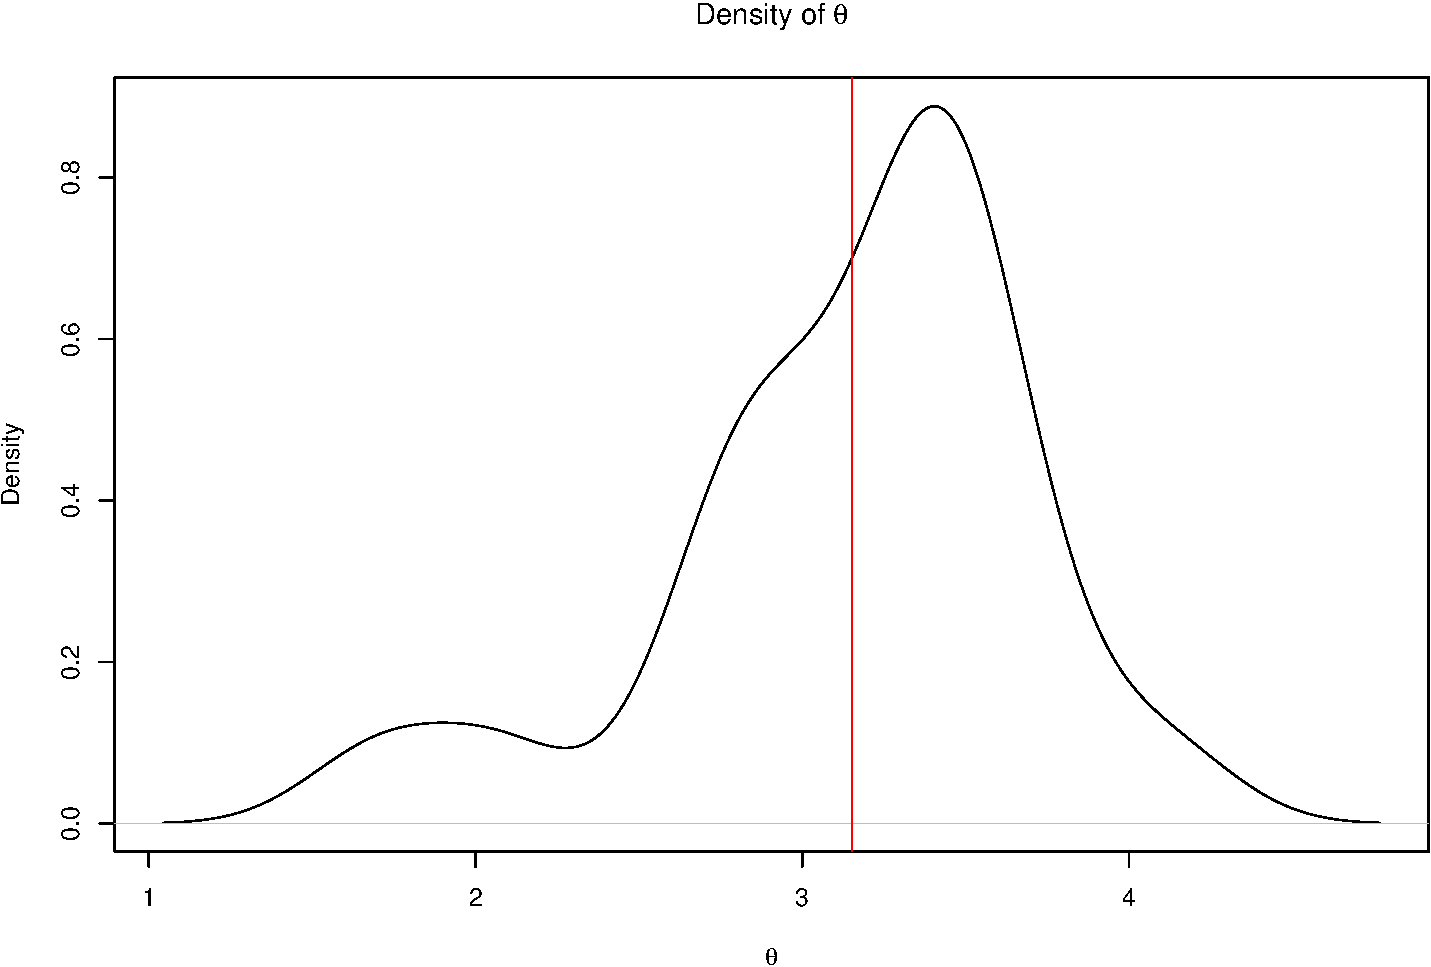
\includegraphics{09-multivariate-norm_v2_files/figure-beamer/unnamed-chunk-12-1.pdf}

\end{frame}

\begin{frame}{Traceplot of \(\theta_2\)}

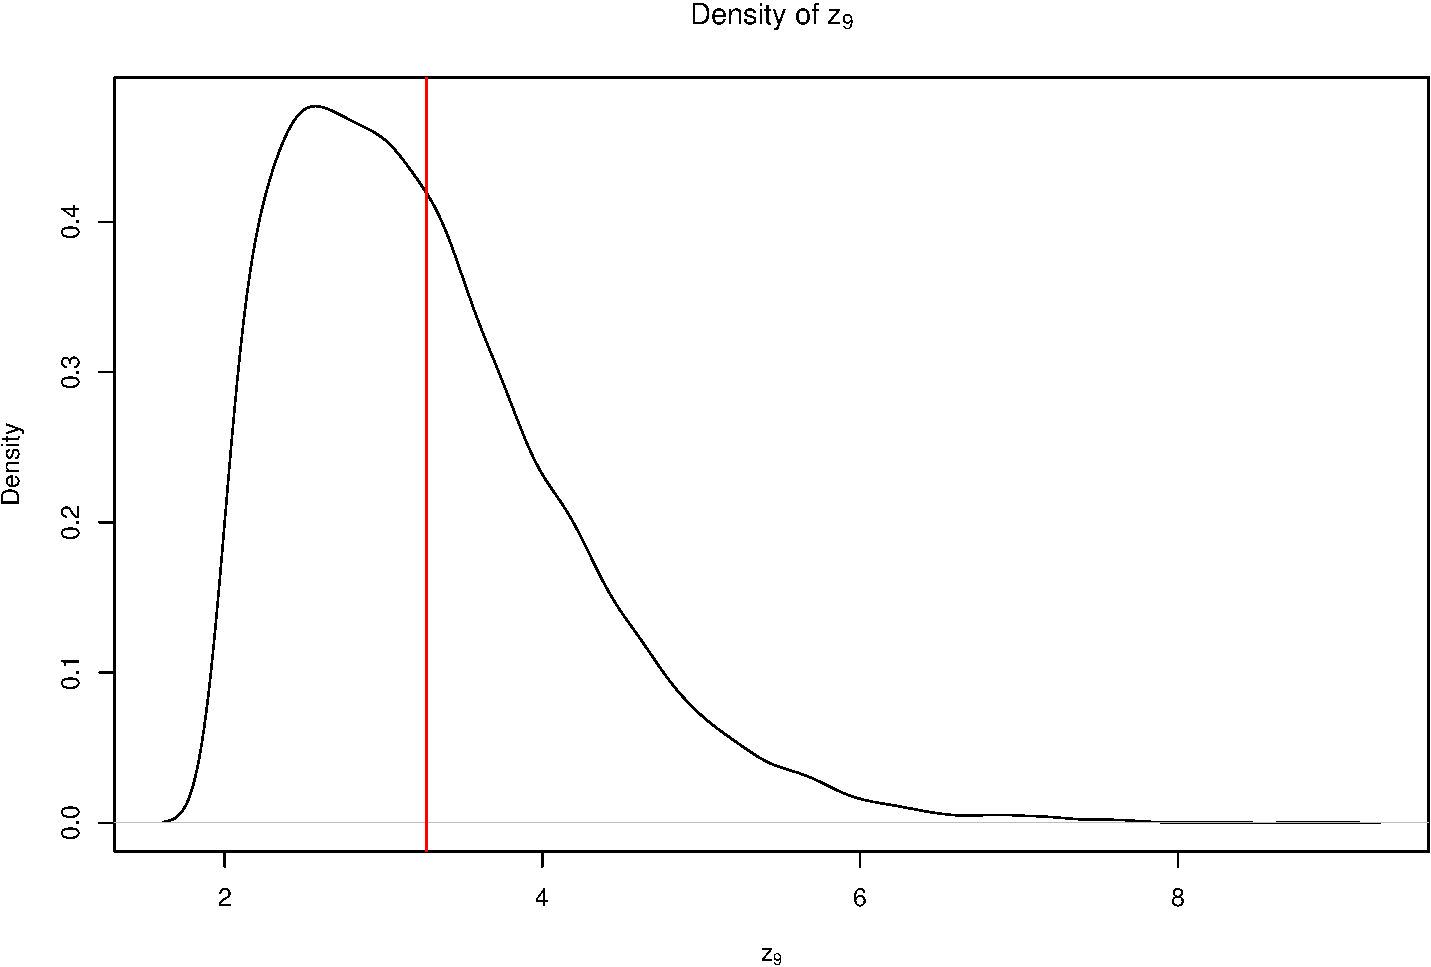
\includegraphics{09-multivariate-norm_v2_files/figure-beamer/unnamed-chunk-13-1.pdf}

\end{frame}

\begin{frame}{Running average plot of \(\theta_1\)}

\includegraphics{09-multivariate-norm_v2_files/figure-beamer/unnamed-chunk-14-1.pdf}

\end{frame}

\begin{frame}{Running average plot of \(\theta_2\)}

\includegraphics{09-multivariate-norm_v2_files/figure-beamer/unnamed-chunk-15-1.pdf}

\end{frame}

\begin{frame}{Estimated density of \(\theta_1\)}

\includegraphics{09-multivariate-norm_v2_files/figure-beamer/unnamed-chunk-16-1.pdf}

\end{frame}

\begin{frame}{Estimated density of \(\theta_2\)}

\includegraphics{09-multivariate-norm_v2_files/figure-beamer/unnamed-chunk-17-1.pdf}

\end{frame}

\begin{frame}{Traceplots and running average plots}

The traceplots don't tell us much of anything, so this is why we examine
the running average plots. Specifically, the traceplots indicate that
the chain has not failed to converged.

The running average plots indicate that the sampler appears to be mixing
well by 5,000 iterations and that the chain has not failed to converged.

\end{frame}

\begin{frame}{Traceplots and running average plots of \(\sigma\)}

Examine the trace plots and running average plots of \(\Sigma\) on your
own.

\end{frame}

\begin{frame}{Return to posterior inference}

Given our samples from our Gibbs sampler, we can approximate posterior
probabilities and confidence regions.

\end{frame}

\begin{frame}[fragile]{Confidence regions}

\begin{Shaded}
\begin{Highlighting}[]
\KeywordTok{quantile}\NormalTok{(THETA[,}\DecValTok{2}\NormalTok{] }\OperatorTok{-}\StringTok{ }\NormalTok{THETA[,}\DecValTok{1}\NormalTok{], }\DataTypeTok{prob=}\KeywordTok{c}\NormalTok{(}\FloatTok{0.025}\NormalTok{,}\FloatTok{0.5}\NormalTok{,}\FloatTok{0.975}\NormalTok{))}
\end{Highlighting}
\end{Shaded}

\begin{verbatim}
##      2.5%       50%     97.5% 
##  1.356260  6.614818 11.667128
\end{verbatim}

\end{frame}

\begin{frame}[fragile]{Posterior inference}

Suppose we were to give the exams/instruction to a large population,
then would the average score on the second exam be higher than the first
second?

We can quanify this by calculating
\[Pr(\theta_2 > \theta_1 \mid y_1,\ldots y_n) = 0.99 
\]

\begin{Shaded}
\begin{Highlighting}[]
\KeywordTok{mean}\NormalTok{(THETA[,}\DecValTok{2}\NormalTok{] }\OperatorTok{>}\StringTok{ }\NormalTok{THETA[,}\DecValTok{1}\NormalTok{])}
\end{Highlighting}
\end{Shaded}

\begin{verbatim}
## [1] 0.9926
\end{verbatim}

\end{frame}

\end{document}
